
\documentclass[paper=a4, fontsize=11pt]{report}

\usepackage[utf8]{inputenc}
\usepackage{titlesec}

\usepackage[numberedsection]{glossaries}

\makeglossaries
 
\newglossaryentry{Persona}
{
        name=Persona,
        description={Is the aspect of someone's character that is presented to or perceived by others}
}
 
\newglossaryentry{Domain Model}
{
        name=Domain Model,
        description={It is a conceptual model of the domain that incorporates both behavior and data}
}
 
\newglossaryentry{Use Case Diagram}
{
        name=Use Case Diagram,
        description={A use case diagram at its simplest is a representation of a user's interaction with the system that shows the relationship between the user and the different use cases in which the user is involved}
}

\newglossaryentry{Activity Diagram}
{
        name=Activity Diagram,
        description={Activity diagrams are graphical representations of workflows of stepwise activities and actions with support for choice, iteration, and concurrency}
}

%%new packages

\usepackage{amsmath}
\usepackage{latexsym}
\usepackage{amsfonts}
\usepackage[normalem]{ulem}
\usepackage{array}
\usepackage{amssymb}
\usepackage{graphicx}
\usepackage[backend=biber,
style=numeric,
sorting=none,
isbn=false,
doi=false,
url=false,
]{biblatex}\addbibresource{bibliography.bib}

\usepackage{subfig}
\usepackage{wrapfig}
\usepackage{wasysym}
\usepackage{enumitem}
\usepackage{adjustbox}
\usepackage{ragged2e}
\usepackage[svgnames,table]{xcolor}
\usepackage{tikz}
\usepackage{longtable}
\usepackage{changepage}
\usepackage{setspace}
\usepackage{hhline}
\usepackage{multicol}
\usepackage{tabto}
\usepackage{float}
\usepackage{multirow}
\usepackage{makecell}
\usepackage{fancyhdr}
\usepackage[toc,page]{appendix}
\usepackage[hidelinks]{hyperref}
\usetikzlibrary{shapes.symbols,shapes.geometric,shadows,arrows.meta}
\tikzset{>={Latex[width=1.5mm,length=2mm]}}
\usepackage{flowchart}\usepackage[paperheight=11.0in,paperwidth=8.5in,left=1in,right=1in,top=0.5in,bottom=0.5in,headheight=1in]{geometry}
\usepackage[utf8]{inputenc}
\usepackage[T1]{fontenc}
\TabPositions{0.5in,1.0in,1.5in,2.0in,2.5in,3.0in,3.5in,4.0in,4.5in,5.0in,5.5in,6.0in,6.5in,7.0in,}

\urlstyle{same}


 %%%%%%%%%%%%  Set Depths for Sections  %%%%%%%%%%%%%%

% 1) Section
% 1.1) SubSection
% 1.1.1) SubSubSection
% 1.1.1.1) Paragraph
% 1.1.1.1.1) Subparagraph


\setcounter{tocdepth}{5}
\setcounter{secnumdepth}{5}


 %%%%%%%%%%%%  Set Depths for Nested Lists created by \begin{enumerate}  %%%%%%%%%%%%%%


\setlistdepth{9}
\renewlist{enumerate}{enumerate}{9}
		\setlist[enumerate,1]{label=\arabic*)}
		\setlist[enumerate,2]{label=\alph*)}
		\setlist[enumerate,3]{label=(\roman*)}
		\setlist[enumerate,4]{label=(\arabic*)}
		\setlist[enumerate,5]{label=(\Alph*)}
		\setlist[enumerate,6]{label=(\Roman*)}
		\setlist[enumerate,7]{label=\arabic*}
		\setlist[enumerate,8]{label=\alph*}
		\setlist[enumerate,9]{label=\roman*}

\renewlist{itemize}{itemize}{9}
		\setlist[itemize]{label=$\cdot$}
		\setlist[itemize,1]{label=\textbullet}
		\setlist[itemize,2]{label=$\circ$}
		\setlist[itemize,3]{label=$\ast$}
		\setlist[itemize,4]{label=$\dagger$}
		\setlist[itemize,5]{label=$\triangleright$}
		\setlist[itemize,6]{label=$\bigstar$}
		\setlist[itemize,7]{label=$\blacklozenge$}
		\setlist[itemize,8]{label=$\prime$}

\setlength{\topsep}{0pt}\setlength{\parskip}{8.04pt}
\setlength{\parindent}{0pt}

\renewcommand{\arraystretch}{1.3}

%%New packages

\usepackage[T1]{fontenc}
\usepackage{fourier}

\usepackage{caption}

\usepackage[english]{babel}															% English language/hyphenation
\usepackage[protrusion=true,expansion=true]{microtype}	
\usepackage{amsmath,amsfonts,amsthm} % Math packages

%%% Custom sectioning
\usepackage{sectsty}
\allsectionsfont{\centering \normalfont\scshape}



%%% Equation and float numbering
\numberwithin{equation}{section}		% Equationnumbering: section.eq#
\numberwithin{figure}{section}			% Figurenumbering: section.fig#
\numberwithin{table}{section}				% Tablenumbering: section.tab#


%%% Maketitle metadata
\newcommand{\horrule}[1]{\rule{\linewidth}{#1}} 	% Horizontal rule

\titleformat{\chapter}{\centering\normalfont\huge}{\thechapter.}{20pt}{\huge}

%%% Begin document
\begin{document}

\begin{titlepage}
    \centering
    \vfill
    
\includegraphics[width=9cm]{Concordia-University-logo.png}
    {\bfseries\Large
        \vskip2cm
        Department of Computer Science and Software Engineering \\
        \vskip2cm
        SOEN 6481: SOFTWARE SYSTEMS REQUIREMENTS SPECIFICATION\\
        \vskip2cm
        Abhishek Rajput\\
        Student ID: 40093879\\
        \vskip9mm
        5 July, 2019\\
    }    
    \vfill
    %
\includegraphics[width=4cm]{Concordia-University-logo.png} 
    \vfill
    \vfill
\end{titlepage}

\tableofcontents

\chapter{Abstract}
This project investigates and describes the concept of Champernowne Constant C\textsubscript{10} which is a transcendental real constant. For base 10, the number is defined by concatenating representations of successive integers i.e. 0.12345678910111213141516...
\vskip1mm
Since it's decimal expansion has important and unique properties, many mathematicians and teachers have found this number profoundly useful. It is constructed in such a way that it's decimal digits are easy to investigate. This allows establishing easily that it is normal in its base.
\vskip1mm
During the project, I have also interviewed two people with strong mathematical background regarding this constant and its application. Moreover, I have created a persona based on the analysis of the interview that was conducted.
\vskip1mm
In this report, I have discussed concepts relevant to Calculator for Champernowne Constant. It includes a description of each concept, relationships between concepts and a Domain Model.
\vskip1mm
Additionally, illustration with the description of each Use Case, Use Case Diagram and Activity Diagram for the Use Cases and UML for the normal scenario of each use case has also been included in this report.


\chapter{Acknowledgement}
I would like to express my deepest appreciation to all those who helped me and provided me the possibility to complete this project.
\vskip1mm
This project would not have been possible without the essential and gracious support of Prof. P. Kamthan whose contribution in stimulating suggestions and encouragement guided me throughout.
\vskip1mm
I would also like to express my sincere gratitude to our Teaching Assistant, Mr. Mehran Ishanian, who had given his assistance to clarify my doubts during this project.
\vskip1mm
Furthermore, I would also like to acknowledge with much appreciation the crucial role of the interviewee Dr. Pankaj Srivastava and Mr. Aayush Sharma, who gave their valuable time from their busy schedule to help me in completion of this project. 
\vskip1mm
Finally, I would like to thank my family and friends for all their understanding and support. 



\chapter{Introduction (Problem 1)}
In mathematics, the Champernowne Constant C\textsubscript{10}, named after economist and mathematician D. G. Champernowne, is a transcendental real constant whose decimal expansion has important properties.\newline
Transcendental numbers are the numbers which are not the root of any polynomial with integer coefficients, i.e., opposite of algebraic numbers.\newline
For base 10, the number is defined by concatenating representations of successive integers:
\[ C\textsubscript{10} = 0.12345678910111213141516... \]  
\begin{flushleft}
Champernowne constants can also be constructed in other bases, similarly, for example:
\end{flushleft}

\[ C\textsubscript{2} = 0.11011100101110111... \]
\[ C\textsubscript{3} = 0.12101112202122... \]

\begin{flushleft}
The Champernowne constants can be expressed exactly as infinite series:
\end{flushleft}

\begin{align*}
{\displaystyle C_{m}=\sum _{n=1}^{\infty }{\frac {n}{10_{b}^{~\left(\sum \limits _{k=1}^{n}\left\lceil \log _{10_{b}}(k+1)\right\rceil \right)}}}}
\end{align*}

\begin{align*}
where\ {\displaystyle \lceil {x}\rceil =} \ ceiling(x), {\displaystyle 10_{b}^{~x}=b^{x}}\ in\ base\ 10,\ {\displaystyle \log _{10_{b}}(x)=\log _{b_{10}}(x)} \ and\  b\ is\ the\ base\ of \ the \ constant.
\end{align*}

\begin{flushleft}
In simpler words, we can say that Champernowne Constant is formed by taking the sequence of whole numbers, i.e., 1, 2, 3, 4, 5, and so on and putting them behind a decimal point.\newline

This constant is interesting because any given sequence of numbers can be shown to exist somewhere in the Champernowne representation.\newline

Another interesting feature of this number is that if a person is picking up a number then there is a 1/10 chance of getting a specific one-digit number, 1/100 chance of getting a specific two-digit number, 1/1000 chance of getting a specific three-digit number and so on.\newline

In other words, for Champernowne Constant, in base 10, we would expect strings [0],[1],[2],...,[9] to occur 1/10 of the time, strings [0,0],[0,1],...,[9,8],[9,9] to occur 1/100 of the time, and so on, which also implies that Champernowne Constant is normal in base 10.
\end{flushleft}

%%Interview Section Starts

\chapter{Interview (Problem 2)}
In this section, I will discuss the interview conducted with the potential users of Champernowne Constant. \newline
It includes criteria for the selection of interviewees, questions asked in the interview, interviewee's responses to the questions and my analysis of this interview process.

\section{Criteria used to select Interviewee}
As Champernowne Constant is famous for its transcendental and normal nature so, in my opinion, a person having a strong background in mathematics would be the most suitable match for being an interviewee.
Keeping this thing in mind, I interviewed below two people over the phone based on my designed questionnaire.

\begin{flushleft}
\textbf{1. Interviewee 1}
\\Name: Dr. Pankaj Srivastava 
\\Qualification: M.Sc Mathematics, Ph.D
\end{flushleft}

\begin{flushleft}
\textbf{2. Interviewee 2}
\\Name: Aayush Sharma 
\\Qualification: M.Sc Mathematics
\end{flushleft}

\section{Interview Questions \& Responses}
\begin{flushleft}
\textbf{Question 1: What is your age?}
\\Response:
\\Interviewee 1: I am 42 years old.
\\Interviewee 2: 30 years old.
\\\hrulefill
\end{flushleft}

\begin{flushleft}
\setlength{\parskip}{\baselineskip}
\textbf{Question 2: What is your current profession?}
\\Response:
\\Interviewee 1: Professor at MNNIT, Allahabad.
\\Interviewee 2: Lecturer at ABES, Ghaziabad.
\\\hrulefill
\end{flushleft}

\begin{flushleft}
\setlength{\parskip}{\baselineskip}
\textbf{Question 3: How much experience do you have in teaching?}
\\Response:
\\Interviewee 1: 11 years.
\\Interviewee 2: 5 years.
\\\hrulefill
\end{flushleft}

\begin{flushleft}
\setlength{\parskip}{\baselineskip}
\textbf{Question 4: What is your qualification?}
\\Response:
\\Interviewee 1: M.Sc in Mathematics, Ph.D.
\\Interviewee 2: M.Sc in Mathematics.
\\\hrulefill
\end{flushleft}

\begin{flushleft}
\setlength{\parskip}{\baselineskip}
\textbf{Question 5: How often do you use electronic devices?}
\\Response:
\\Interviewee 1: Very often, I think now life would be quite difficult without the involvement of electronic devices.
\\Interviewee 2: For most of my work.
\\\hrulefill
\end{flushleft}

\begin{flushleft}
\setlength{\parskip}{\baselineskip}
\textbf{Question 6: How would you define Champernowne Constant?}
\\Response:
\\Interviewee 1: A number having a sequence of positive integers after a decimal.
\\Interviewee 2: Simply a decimal following with positive integers numbers till any number of places.
\\\hrulefill
\end{flushleft}

\begin{flushleft}
\setlength{\parskip}{\baselineskip}
\textbf{Question 7: What is the first thing that comes to your mind when you hear about Champernowne Constant?}
\\Response:
\\Interviewee 1: Number having transcendental and normal number properties.
\\Interviewee 2: Normal number.
\\\hrulefill
\end{flushleft}

\begin{flushleft}
\setlength{\parskip}{\baselineskip}
\textbf{Question 8: How is this normal number different from other normal numbers?}
\\Response:
\\Interviewee 1: As far as I know, because this number is normal in both base 2 and 10.
\\Interviewee 2: Well, not very sure about that.
\\\hrulefill
\end{flushleft}

\begin{flushleft}
\setlength{\parskip}{\baselineskip}
\textbf{Question 9: Have you ever used this number in your career?}
\\Response:
\\Interviewee 1: Not many times, but yes, sometimes to give an example of the transcendental and normal number to my students.
\\Interviewee 2: Never used, but have read about it.
\\\hrulefill
\end{flushleft}

\begin{flushleft}
\setlength{\parskip}{\baselineskip}
\textbf{Question 10: Do you know of any application which uses this number? }
\\Response:
\\Interviewee 1: I read that this number can trick any program which attempts to find regularity in sequences.
\\Interviewee 2: Not very sure about it.
\\\hrulefill
\end{flushleft}

\begin{flushleft}
\setlength{\parskip}{\baselineskip}
\textbf{Question 11: Do you know of any field in which it could prove its worth?}
\\Response:
\\Interviewee 1: In my teaching field for sure.
\\Interviewee 2: In the education field, to show what are transcendental and normal numbers.
\\\hrulefill
\end{flushleft}

\begin{flushleft}
\setlength{\parskip}{\baselineskip}
\textbf{Question 12: Can we use this number in combination with any other number to perform some useful tasks?}
\\Response:
\\Interviewee 1: As we get this number after concatenating positive integers after a decimal point  so if we multiply this number with 1 having leading 0s equal to digits after the decimal places then 
we can eventually get a number having digits as the sequence of positive integers.
\\Interviewee 2: No idea.
\\\hrulefill
\end{flushleft}

\begin{flushleft}
\setlength{\parskip}{\baselineskip}
\textbf{Question 13: If I build a calculator to calculate this number what features would you like to be present in that calculator?}
\\Response:
\\Interviewee 1: As this number is normal, your calculator should provide the functionality to find the occurrences of a certain number in this constant and should provide other similar kinds of functionalities as well.
\\Interviewee 2: To get this number up-to any limit.
\\\hrulefill
\end{flushleft}

\begin{flushleft}
\setlength{\parskip}{\baselineskip}
\textbf{Question 14: Could you please tell me any other feature that can make this calculator more useful?}
\\Response:
\\Interviewee 1: You could probably add the functionality to generate graphs of the results obtained. As you know, graphs give a better visualization of results.
\\Interviewee 2: If possible, compute other irrational numbers too.
\\\hrulefill
\end{flushleft}

\begin{flushleft}
\setlength{\parskip}{\baselineskip}
\textbf{Question 15: How can this calculator be useful to you?}
\\Response:
\\Interviewee 1: If I can prove to my students why this number is a normal number, it would definitely be useful for me.
\\Interviewee 2: To generate this number of any length.
\\\hrulefill
\end{flushleft}

\begin{flushleft}
\setlength{\parskip}{\baselineskip}
\textbf{Question 16: How many digits after the decimal should be generated by the calculator for this number?}
\\Response:
\\Interviewee 1: You should give the user the flexibility to enter the precision level.
\\Interviewee 2: I think it should be user-dependent.
\\\hrulefill
\end{flushleft}

\begin{flushleft}
\setlength{\parskip}{\baselineskip}
\textbf{Question 17: In that calculator, would you like to get the result in different formats?}
\\Response:
\\Interviewee 1: I don't think there is any need for that.
\\Interviewee 2: Why not, if possible.
\\\hrulefill
\end{flushleft}

\begin{flushleft}
\setlength{\parskip}{\baselineskip}
\textbf{Question 18: What inputs would you want to give to the calculator in order to generate this number?}
\\Response:
\\Interviewee 1: I think just the precision level should be enough.
\\Interviewee 2: Base and number of digits after the decimal.
\\\hrulefill
\end{flushleft}

\begin{flushleft}
\setlength{\parskip}{\baselineskip}
\textbf{Question 19: How would you like to use this calculator (Console or UI)?}
\\Response:
\\Interviewee 1: Either way, but a calculator with UI would be easier to use.
\\Interviewee 2: UI, for sure.
\\\hrulefill
\end{flushleft}

\begin{flushleft}
\setlength{\parskip}{\baselineskip}
\textbf{Question 20: If I choose to build a calculator with UI, what things should be kept in mind to have a good UX?}
\\Response:
\\Interviewee 1: Good placement of buttons.
\\Interviewee 2: Number should be displayed properly, proper alignment of components, good color contrast.
\\\hrulefill
\end{flushleft}

\section{Conclusion}
\begin{flushleft}
From this interview, I have concluded the below points:

1. This number is mostly popular for its normal behavior.
\\2. This number can trick programs which attempts to find regularity in sequences.
\\3. The number of places to display after the decimal in the calculator should be dependent on the user's input.
\\4. It is better to have UI for this calculator.
\\5. For additional functionality, you can add 'Generate Graph Functionality'.
\\6. We can use this number to find the position of any number in the string made of a sequence of positive integers.
\\7. We can also use this number to answer questions like- how many digits are there in total in the two-digit numbers 10 to 99, find all the positions at which a string occurs, compute the position at which a given number (a string of digits) first appears in the sequence, number of occurrences of a certain number, etc.

\end{flushleft}
%% Interview section ends

%%Persona Section starts

\chapter{\gls{Persona} (Problem 3)}
\vspace{\baselineskip}



\begin{table}[H]
 			\centering
\begin{tabular}{p{1.86in}p{4.23in}}
\hline

\multicolumn{1}{|p{1.86in}}{
	\begin{Center}
		
\includegraphics[width=1.86in,height=1.8in]{teacher.jpg}
	\end{Center}
 \par } & 
\multicolumn{1}{|p{4.23in}|}{{\fontsize{10pt}{12.0pt}\selectfont \textbf{Personal Information}} \par \begin{itemize}
	\item {\fontsize{10pt}{12.0pt}\selectfont \textbf{Name}: Rahul Sharma} \par 	\item {\fontsize{10pt}{12.0pt}\selectfont \textbf{Job} \textbf{Title}: Teacher} \par 	\item {\fontsize{10pt}{12.0pt}\selectfont \textbf{Age}: 35 years} \par 	\item {\fontsize{10pt}{12.0pt}\selectfont \textbf{University}: SVNIT, Surat} \par 	\item {\fontsize{10pt}{12.0pt}\selectfont \textbf{Email}: rahul@persona.com} \par 	\item {\fontsize{10pt}{12.0pt}\selectfont \textbf{Location}: India}
\end{itemize} \par } \\
\hhline{--}

\multicolumn{2}{|p{6.29in}|}{{\fontsize{10pt}{12.0pt}\selectfont \textbf{Skills}} \par \begin{itemize}
	\item {\fontsize{10pt}{12.0pt}\selectfont Basic hypergeometric functions} \par 	\item {\fontsize{10pt}{12.0pt}\selectfont Tensor analysis} \par 	\item {\fontsize{10pt}{12.0pt}\selectfont Fuzzy theory} \par 	\item {\fontsize{10pt}{12.0pt}\selectfont Cryptography } \par 	\item {\fontsize{10pt}{12.0pt}\selectfont Market research}
\end{itemize} \par } \\
\hhline{--}

\multicolumn{2}{|p{6.29in}|}{{\fontsize{10pt}{12.0pt}\selectfont \textbf{Experience}} \par {\fontsize{10pt}{12.0pt}\selectfont \vskip1mm He has an experience of 11 years in the teaching profession and has a strong inclination towards the results about the combination of irrational numbers.} \par } \\
\hhline{--}

\multicolumn{2}{|p{6.29in}|}{{\fontsize{10pt}{12.0pt}\selectfont \textbf{User requirements}} \par \begin{itemize}
	\item {\fontsize{10pt}{12.0pt}\selectfont Generate Champernowne Constant (C\textsubscript{10})} \par 	\item {\fontsize{10pt}{12.0pt}\selectfont Perform some basic calculations} \par 	\item {\fontsize{10pt}{12.0pt}\selectfont Obtain a number of occurrences of a particular digit in generated Champernowne Constant} \par 	\item {\fontsize{10pt}{12.0pt}\selectfont Obtain the place of a particular number in generated Champernowne Constant} \par 	\item {\fontsize{10pt}{12.0pt}\selectfont Obtain frequency of numbers}
\end{itemize} \par } \\
\hhline{--}

\multicolumn{2}{|p{6.29in}|}{ \par {\fontsize{10pt}{12.0pt}\selectfont \textbf{Goals \tabto{1.54in} }} \par  \par {\fontsize{10pt}{12.0pt}\selectfont \vskip1mm He wants to generate Champernowne Constant with the variable number of places after the decimal point and would also like to do some basic calculations along with finding occurrences of a digit and place of a number.}} \\
\hhline{--}

\end{tabular}
 \end{table}




\vspace{\baselineskip}

%%Persona ends

%%Domain Model Starts
\chapter{\gls{Domain Model} (Problem 4)}
In this section, I will discuss about Concepts relevant to Calculator for Champernowne Constant. \newline
It includes a description of each Concepts, relationships between Concepts and finally a Domain Model.
  
\section{Different Concepts relevant to calculator for Champernowne Constant  }

\begin{flushleft}
\textbf{1: User}
\\Description - This is the Concept which will get benefited from using the Calculator.
\\Attributes:
\\A. name - Name of the person using the Calculator.
\end{flushleft}

\begin{flushleft}
\setlength{\parskip}{\baselineskip}
\textbf{2: Button}
\\Description - Button is a medium to provide inputs to the Calculator. This is a generalization for NumberButton and ActionButton.
\\Attributes:
\\A. buttonID - Unique identifier for Button.
\\B. buttonColor - Color of the Button.
\\C. buttonSize - Size of Button on Calculator layout.
\\D. buttonCoordinates - Position of Button on Calculator layout.
\end{flushleft}

\begin{flushleft}
\textbf{3: NumberButton}
\\Description - This is the specialization of Button class.
\\Attributes:
\\A. numberDisplayed - Number to be displayed on the Button. This is also the number which will be input to the Calculator. 
\end{flushleft}

\begin{flushleft}
\textbf{4: ActionButton}
\\Description - This is the specialization of Button class.
\\Attributes:
\\A. actionDisplayed - Action name to be displayed on the Button. This is also the name of the action which will get performed on pressing this Button.
\end{flushleft}

\begin{flushleft}
\textbf{5: InputField}
\\Description - Like Button, Input field is another medium to provide inputs to the Calculator.
\\Attributes:
\\A. fieldID - Unique identifier for InputField.
\\B. filedSize - Size of Field on Calculator layout.
\\C. fieldCoordinates - Position of Field on Calculator layout.
\\D. fieldFontStyle - Font type used in the Field.
\\E. fieldFontSize - Size of the font used in the Field.
\\F. inputMaxSize - Maximum length of the input to the Field.
\end{flushleft}
\pagebreak

\begin{flushleft}
\textbf{6: Output   }
\\Description - Output is the result obtained after interacting with the Calculator. Output is also the generalization for SpecialNumber.
\\Attributes:
\\A. size: Length of the output.
\end{flushleft}

\begin{flushleft}
\textbf{7: OutputArea}
\\Description - OutputArea will be used to display the results post performing any actions on the Calculator.
\\Attributes:
\\A. areaID - Unique identifier for output Area.
\\B. areaSize - Size of Area on Calculator layout.
\\C. areaCoordinates - Position of Area on Calculator layout.
\\D. areaFontStyle - Font type used in the Area.
\\E. areaFontSize - Size of the font used in the Area.
\\F. outputMaxSize - Maximum length of the output to the Area.
\end{flushleft}

\begin{flushleft}
\textbf{8: InstructionPane   }
\\Description - InstructionPane will be used to display the instructions on how to use the Calculator to the user.
\\Attributes:
\\A. paneID - Unique identifier for instruction Pane.
\\B. paneSize - Size of Pane on Calculator layout.
\\C. paneCoordinates - Position of Pane on Calculator layout.
\\D. paneFontStyle - Font type used in the Pane.
\\E. paneFontSize - Size of font the used in the Pane.
\\F. paneMaxSize - Maximum length of the instructions on the Pane.

\end{flushleft}

\begin{flushleft}
\textbf{9: SpecialNumber   }
\\Description - SpecialNumber is the specialization of Output. SpecialNumber will contain the information related to the Champernowne Constant.
\\Attributes:
\\A. decimalPlaces: Length of the output.
\end{flushleft}

\section{Relationship between Concepts  }

\begin{flushleft}
\textbf{1: presses}
\\Between - User and Button
\\Explanation: This relationship shows that a user can interact with Calculator by pressing one or more buttons.
\end{flushleft}

\begin{flushleft}
\textbf{2: populates}
\\Between - Button and InputField
\\Explanation: This relationship shows that one or more buttons will populate the input field which then will be used to as inputs to perform the calculation.
\end{flushleft}

\begin{flushleft}
\textbf{3: generates}
\\Between - ActionButton and Output
\\Explanation: This relationship shows that one action button will generate one or more outputs after processing the inputs present in the input field.
\end{flushleft}

\begin{flushleft}
\textbf{4: displayedOn}
\\Between - Output and OutputArea
\\Explanation: This relationship shows that one or more outputs/results will be displayed on one OutputArea.
\end{flushleft}

\begin{flushleft}
\textbf{5: shows}
\\Between - OutputArea and SpecialNumber
\\Explanation: This relationship shows that one OutputArea will show one Special Number on the screen.
\end{flushleft}

\begin{flushleft}
\textbf{6: instructs}
\\Between - InstructionPane and User
\\Explanation: This relationship shows that one InstructionPane will instruct one or more users about the inst to use the Calculator in order to get the desired output.
\end{flushleft}

\pagebreak
\begin{figure}[htp]
    \centering
    \vspace{2cm}
    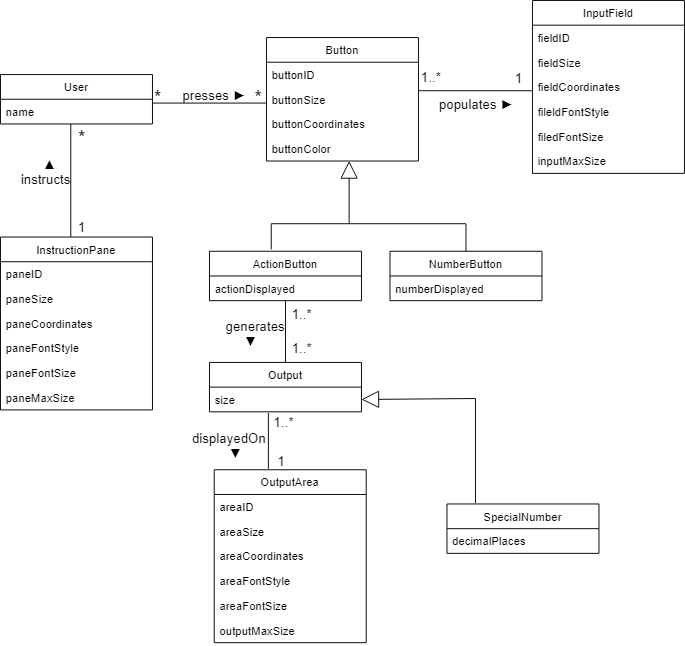
\includegraphics[width=15cm]{DomainModel.png}
    \caption*{\textbf{Fig 1: Domain Model}}
\end{figure}
\pagebreak

%%Domain Model section ends

%%Use Case Model section starts
\chapter{Use Case Model (Problem 5)}
In this section, I will discuss about Use Cases relevant to Calculator for Champernowne Constant. \newline
It includes a description of each Use Case, \gls{Use Case Diagram} and \gls{Activity Diagram} for the Use Cases and UML for the normal scenario of each use case.
  
\section{Use Cases relevant to calculator for Champernowne Constant  }

\begin{flushleft}
\textbf{UC1: Generate Number }
\\Description - This use case includes 'Display Result' use case. This use case is responsible for generating Champernowne Constant up-to-the places desired by the user.
\end{flushleft}

\begin{flushleft}
\textbf{UC2: Perform Calculation }
\\Description - This use includes 'Display Result' use case and extended by 'Get Occurrences' and 'Get Number Place' use cases. This use case is responsible for performing the calculation based on user inputs and display the results.
\end{flushleft}

\begin{flushleft}
\textbf{UC3: Display Results }
\\Description - This use is included in 'Generate Number' and 'Perform Calculation' use cases. This is responsible for displaying the results to the user in the output screen.
\end{flushleft}

\begin{flushleft}
\textbf{UC4: Get Occurrences}
\\Description - This use case is the specialization of 'Perform Calculation' use case. This use case case is responsible for calculating the number of occurrences of a particular number in the generated number.
\end{flushleft}

\begin{flushleft}
\textbf{UC5: Get Number Place }
\\Description -This use case is the specialization of 'Perform Calculation' use case. This use case is responsible for calculate the position of first occurrence of a particular number in generated Champernowne Constant.
\end{flushleft}

\begin{flushleft}
\textbf{UC6: Edit Input Field }
\\Description - This use case gives the user the option to insert or edit the values in the Input field.
\end{flushleft}

\begin{flushleft}
\textbf{UC7: Clear Input Field  }
\\Description - This use case includes 'Edit Input Field' use case. This use case clears the input field.
\end{flushleft}

\begin{flushleft}
\textbf{UC8: Store Result }
\\Description - This use case is responsible for storing the result so that it can be used at a later time, if needed.
\end{flushleft}

\begin{flushleft}
\textbf{UC9: Retrieve Result}
\\Description - This use case includes 'Edit Input Field' use case. This use case is responsible for retrieving the value stored by 'Store Result' use case and populate the Input field using retrieved value. 
\end{flushleft}

\pagebreak
\begin{figure}[htp]
    \centering
    \vspace{2cm}
    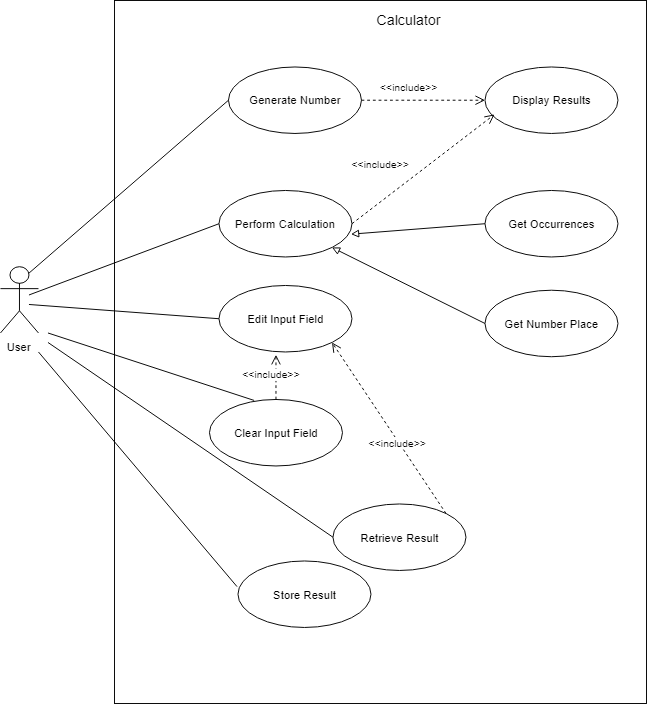
\includegraphics[width=15cm]{UseCaseDiagram.png}
    \caption*{\textbf{Fig 2: Use Case Diagram}}
\end{figure}

\pagebreak
\begin{figure}[htp]
    \centering
    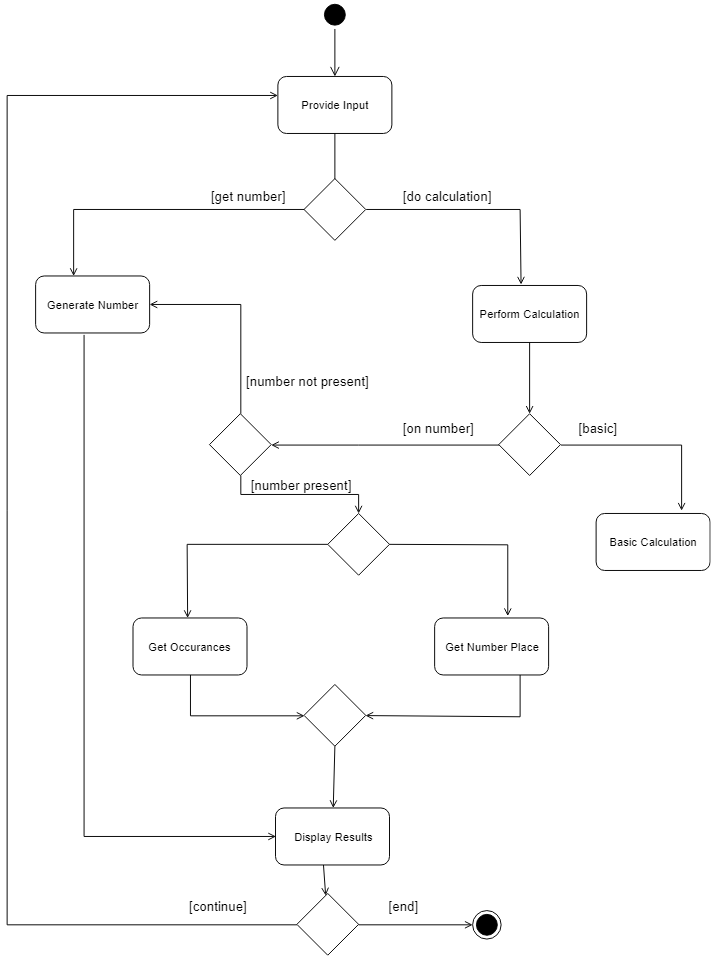
\includegraphics[width=15cm]{ActivityDiagram.png}
    \caption*{\textbf{Fig 3: Activity Diagram}}
\end{figure}

\pagebreak
\begin{figure}[htp]
    \centering
    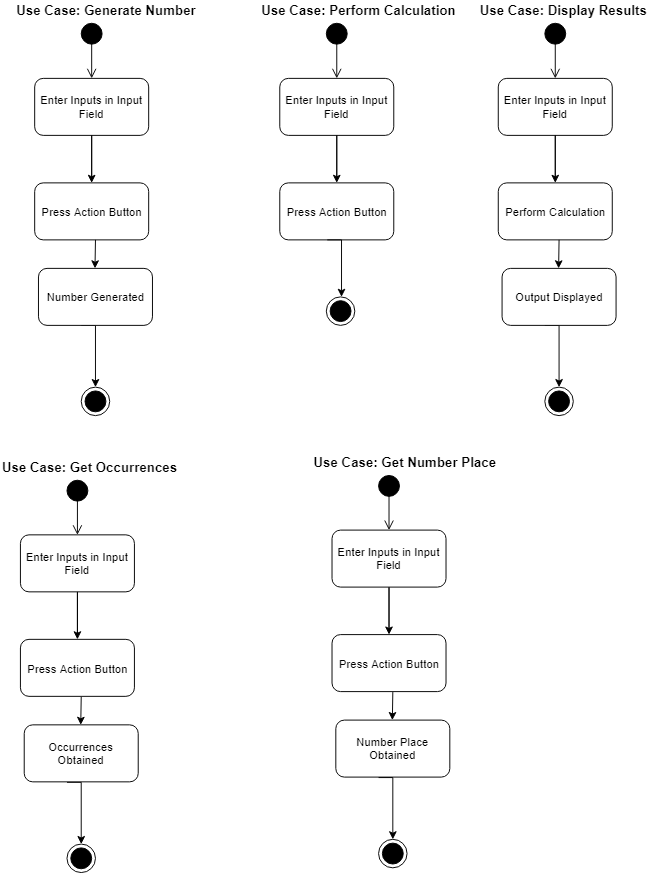
\includegraphics[width=15cm]{NormalScenario1.png}
    \caption*{\textbf{Fig 4.1: Normal Scenario for Use Cases}}
\end{figure}

\pagebreak
\begin{figure}[htp]
    \centering
    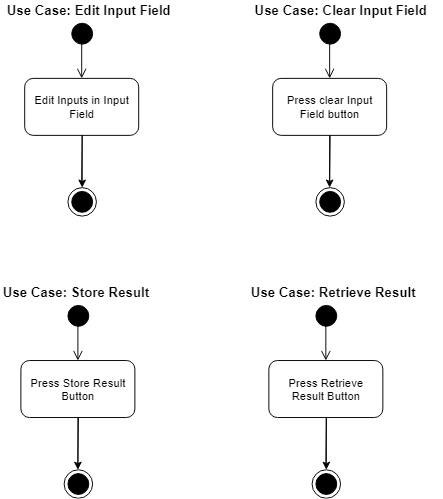
\includegraphics[width=15cm]{NormalScenario2.png}
    \caption*{\textbf{Fig 4.2: Normal Scenario for Use Cases}}
\end{figure}

%%Use case model ends


%%User Stories starts

\chapter{User Stories (Problem 6)}
In this section, I will cover user stories relevant to Calculator for Champernowne Constant. \newline

  
\section{User Stories relevant to calculator for Champernowne Constant }

\begin{center}
\begin{tabular}{| m{1.3cm} | m{27em} | m{4cm}| m{1.2cm} | m{1.2cm} |} 
\hline
Identifier & User Stories & Constraint & Priority & Estimate \\ [0.7ex]
\hline\hline
US1 & As a user, I want to generate the Champernowne Constant. & Performance, Correctness, Readability & 5 & 5 \\ 
\hline
US2 & As a user, I want to choose the number of digits after the decimal point in generated Champernowne Constant. & Field validation, Modifiability & 4 & 3 \\ 
\hline
US3 & As a user, I want to calculate the number of occurrences of a particular number in generated Champernowne Constant. & Performance, Correctness, Reliability & 4 & 5 \\ 
\hline
US4 & As a user, I want to calculate the position of the first occurrence of a particular number in generated Champernowne Constant. & Performance, Correctness, Reliability & 4 & 5 \\ 
\hline
US5 & As a user, I want to store the result, to use it at a later time, if needed. & Reusability & 2 & 2 \\ 
\hline
US6 & As a user, I want to retrieve the stored result, whenever needed. & Readability, Operability & 2 & 2 \\ 
\hline
US7 & As a user, I want to delete the content of the input field one by one, from end. & Modifiability & 3 & 1 \\ 
\hline
US8 & As a user, I want to clear the content of the input field. & Modifiability & 3 & 1 \\ 
\hline
US9 & As a user, I want to clear the content of the output screen. & Modifiability & 2 & 1 \\ 
\hline
US10 & As a user, I want to do basic calculations: Addition, Subtraction, Multiplication, and Division. & Performance, Correctness, Readability & 4 & 4 \\ 
\hline
US11 & As a user, I want to insert values in input field, either using calculator keys or using a keyboard or both. & Reliability, Operability & 5 & 4 \\ 
\hline
\end{tabular}
\end{center}

\section{Acceptance Criteria for User Stories }

\begin{center}
\begin{tabular}{| m{1.3cm} |  m{1.2cm} | m{35em} |} 
\hline
S. No. & User Stories & Acceptance Tests \\ [0.7ex]
\hline\hline
1 & US1 & a). Must be in base 10.\newline
b). Must have a decimal point at second place.\newline
c). Complete number must be readable.\newline
d). Number must get displayed within 5 seconds. \\ 
\hline
2 & US2 & a). Number of digits entered must be integer only. \\ 
\hline
3 & US3 & a). Occurrences obtained must be for the entered number only.\newline
b). The result must get displayed within 5 seconds. \\ 
\hline
4 & US4 & a). Position obtained must be for the entered number only.\newline
b). The position displayed must be of the first occurrence only.\newline
c). The result must get displayed within 5 seconds.  \\ 
\hline
5 & US5 & a). User must get the confirmation regarding the operation. \\ 
\hline
6 & US6 & a). User must get the stored result only. \\ 
\hline
7 & US7 & a). Only one input must get deleted at a time. \\ 
\hline
8 & US8 & a). Input field must get cleared at once. \\ 
\hline
9 & US9 & a). Output screen must get cleared at once. \\ 
\hline
10 & US10 & a). Results must be correct.\newline
b). The result must get displayed within 5 seconds.  \\ 
\hline
11 & US11 & a). User must be able to provide inputs using both keyboard and keypad available on the screen.   \\ 
\hline
\end{tabular}
\end{center}

%%User stories ends

%% traceability matrix starts

\chapter{Backward Traceability Matrix (Problem 7)}
In this section, I will cover backward traceability matrix relevant to Calculator for Champernowne Constant. \newline

  
\section{Backward Traceability Matrix relevant to calculator for Champernowne Constant }

\begin{center}
\begin{tabular}{| m{.8cm} | m{1.8cm} | m{.8cm} | m{.8cm}| m{3cm} | m{1cm} | m{3cm} | m{1.5cm} |} 
\hline
S. No. & User Stories & UC & US & Interview & Survey & Global & Persona \\ [0.7ex]
\hline\hline
1. & US1 & UC1 &  &  &  &  & \\ 
\hline
2 & US2 &  &  & Question: 16, 18 &  &  &   \\ 
\hline
3 & US3 & UC4 &  & Question: 13 &  &  &  \\ 
\hline
4 & US4 & UC5 &  & Question: 13 &  &  &  \\ 
\hline
5 & US5 & UC8 &  &  &  &  &  \\ 
\hline
6 & US6 & UC9 & US5 &  &  &  &  \\ 
\hline
7 & US7 & UC6 &  &  &  & Windows Calculator &  \\ 
\hline
8 & US8 & UC7 &  &  &  & Windows Calculator & \\ 
\hline
9 & US9 &  &  &  &  & Windows Calculator &  \\ 
\hline
10 & US10 & UC2 &  &  &  & Windows Calculator &  \\ 
\hline
11 & US11 &  &  &  &  & Windows Calculator &  \\ 
\hline
\end{tabular}
\end{center}

%% traceability matrix ends


%%Glossary section starts
\printglossary

%%References section starts
\chapter{References}

https://en.wikipedia.org/wiki/Champernowne\_constant
\vskip1mm
http://mathworld.wolfram.com/ChampernowneConstant.html
\vskip1mm
\textbf{GitHub Project Workspace Address:} \url{https://github.com/ariesabhi55/SOEN6481TeamFProject} 
%%% End document
\end{document}
